\chapter{Funktionsweise der Komponenten}\label{ch:funktionsweise_der_komponenten}
Die folgenden Abschnitte beschreiben die Funktionsweise der Mustererkennung in Vuforia und bieten einen grundlegenden Überblick über den Aufbau einer Unity-Anwendung.
\section{Mustererkennung in Vuforia}
Vuforia ist ein Augmented Reality Software Development Kit für die Erstellung von Augmented Reality (AR) Anwendungen auf mobilen Geräten und Tablets.
Verschiedene Ziele können in Echtzeit erkannt und verfolgt werden, was die Möglichkeit bietet, virtuelle Objekte wie 3D Modelle in Bezug auf diese Ziele in der realen Welt zu positionieren.
Das virtuelle Objekt verfolgt dann die Position und Ausrichtung des Bildes in Echtzeit, sodass die Perspektive des Betrachters erhalten und das virtuelle Objekt als ein Teil der realen Szene erscheint.
Das Vuforia SDK unterstützt eine Vielzahl von 2D- und 3D-Zieltypen, einschließlich „markerloser“ Bildziele und eine Form von adressierbaren Referenzmarken, die als \textquote{VuMark} bezeichnet werden. 
Für das beschriebene IT Projekt war die performante Nutzung von zweidimensionalen Bildzielen ausreichend, da nur auf dem Globus angebrachte Markierungen erkannt werden mussten.

Vuforia bietet über eine Schnittstelle zur Unity Game Engine sowohl die Möglichkeit der nativen AR-Entwicklung für iOS und Android, als auch die Möglichkeit der Entwicklung von AR-Anwendungen in Unity, die anschließend auf beide Plattformen portierbar sind.

Das Architekturmodell \ref{fig:vuforia_architektur} beschreibt die Funktionsweise des Vuforia SDKs im Zusammenspiel mit der Unity Engine.

\begin{figure} [h]
\centering
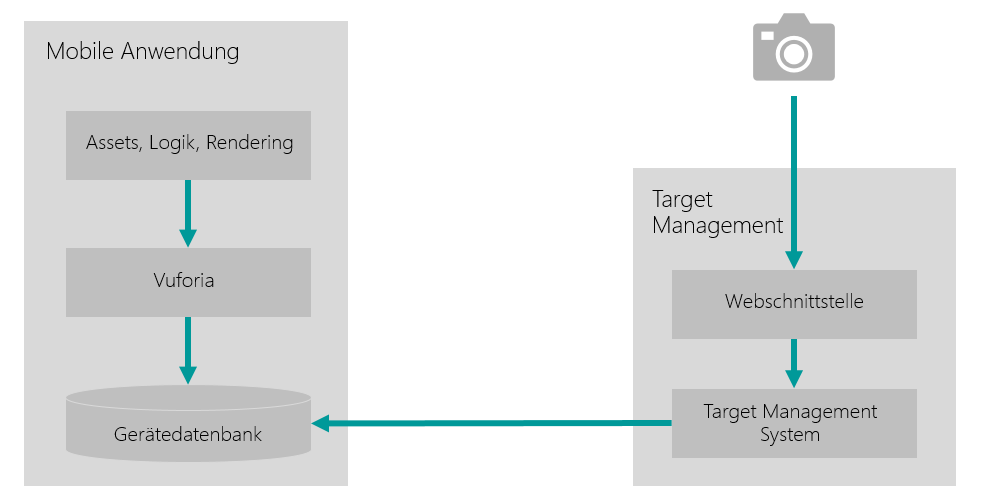
\includegraphics[width=14cm]{vuforia_architektur.PNG}
\caption{Funktionsweise von Vuforia}
\label{fig:vuforia_architektur}
\end{figure}
 
Um Bildziele für die spätere Verwendung in Unity zu generieren, muss der Benutzer selbstgewählte Bilder über die Weboberfläche des \textquote{Target Management Systems} in das System laden.
Bei der Erstellung eines solchen Image Targets ist die Angabe eines Bildnamens und einer Referenzgröße erforderlich, welche sich an der tatsächlichen Größe der verwendeten Marker orientiert.
Das Target Management System liefert dem Nutzer eine Bewertung der erwarteten Erkennungs- und Verfolgungsleistung des Ziels, sowie eine Visualisierung der von der Vuforia Engine verwendeten Merkmale des Ziels, beispielhaft dargestellt in Abbildung \ref{fig:image_target_rating}.
Um ein hohes Rating und somit eine gute Bilderkennung zu gewährleisten, sollte deshalb auf die Wahl von geeigneten Image Targets geachtet werden.
Die Kriterien bei dieser Auswahl werden in Abschnitt \ref{image_targets} beschrieben.

\begin{figure} [h]
\centering
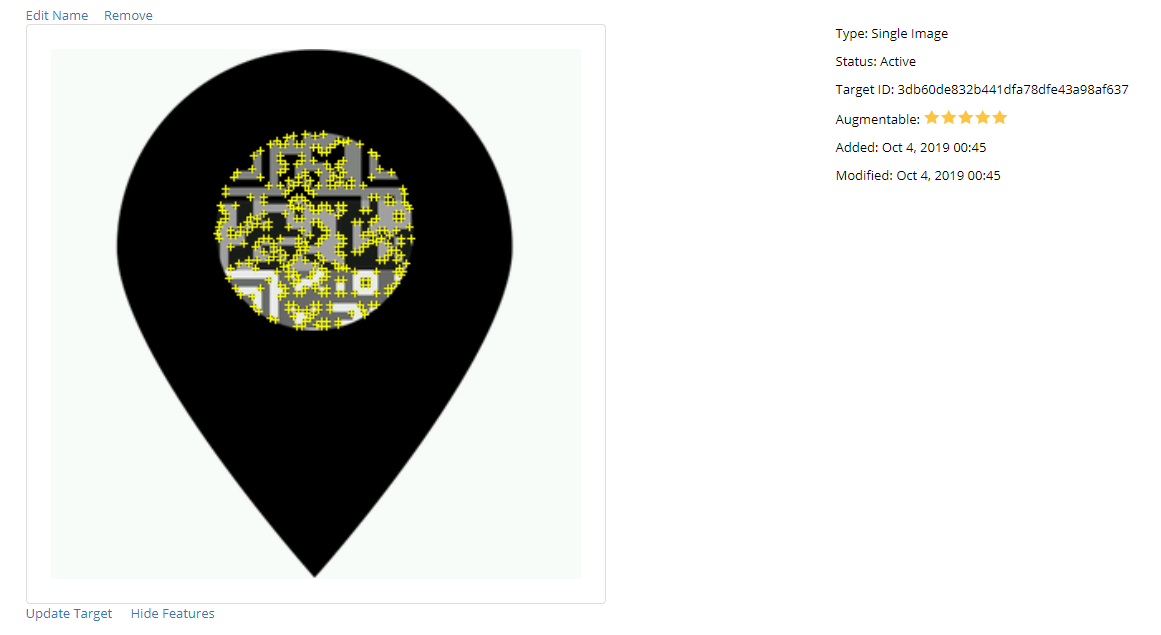
\includegraphics[width=14cm]{image_target_rating.PNG}
\caption{Image Target mit verwendeten Merkmalen und Rating}
\label{fig:image_target_rating}
\end{figure}
 
Das generierte Target Management System kann in Unity importiert werden, sodass die enthaltenen Image Targets in der Gerätedatenbank hinterlegt werden. 
Über das Vuforia SDK, welches in Unity eingebunden sein muss, kann innerhalb der Anwendung auf die Inhalte der Gerätedatenbank zugegriffen werden, um das Kamerabild mit den dort hinterlegten Image Targets zu vergleichen.

Beim Ausführen der Applikation wird dann von der Vuforia Engine eine Mustererkennung durchgeführt und die Kamerainformationen des Gerätes werden mit den in den Gerätedatenbank abgelegten Dateien verglichen. 
Im Falle einer Übereinstimmung wird eine zweite Mustererkennung gestartet, die den Abstand und die Rotation des Musters, welches in der Datenbank gespeichert ist, mit dem erkannten Muster vergleicht.
Diese Informationen verwendet die Vuforia Engine dann, um die Größe und Ausrichtung des darzustellenden 3D Modells entsprechend anzupassen. (vgl. \cite{Grahn2017})
\section{Aufbau einer Unity-Applikation}